% !TEX encoding = UTF-8 Unicode

\documentclass[a4paper]{article}

\usepackage{color}
\usepackage{url}
\usepackage[T2A]{fontenc} 
\usepackage[utf8]{inputenc}
\usepackage{graphicx}

\usepackage[english,serbian]{babel}
\usepackage[unicode]{hyperref}
\hypersetup{colorlinks,citecolor=green,filecolor=green,linkcolor=blue,urlcolor=blue}

\begin{document}

\title{Kriptovalute\\ \small{Seminarski rad u okviru kursa\\Računarstvo i društvo\\ Matematički fakultet}}

\author{Petar Rondović\\ mi17167@alas.matf.bg.ac.rs}
\date{~Septembar 2022.}
\maketitle

\abstract{
Ovaj rad objašnjava šta su i kako funkcionišu kriptovalute. Prolazi kroz tehnologije i tehnike na kojima je baziran ceo sistem kriptovaluta i ukazuje u koje još svrhe se mogu upotrebiti. Ukratko se spominju osnovni koncepti razvoja novca, navodi se nekoliko primera kriptovaluta i njihove karakteristike.
\tableofcontents

\newpage

\section{Uvod}
\label{sec:uvod}
Kriptovalute su tip valute koje postoje digitalno i koriste kriptografiju za zaštitu transakcija. One nemaju centralni organ za izdavanje ni za regulisanje nego umesto toga koriste decentralizovani sistem za zapisivanje transakcija i izdavanje novih jedinica kriptovalute \cite{kriptovalute1}. Prva kriptovaluta, \emph{Bitcoin}, nastala je 2009. za vreme najhaotičnijeg perioda u istoriji SAD-a. Za vreme globalne finansijske krize od 2007. do 2009. nepoverenje u banke i centralne vlade bilo je na vrhuncu. U takvim okolnostima raste poularnost decentralizovanog sistema plaćanja koji ne zavisi od državne uprave \cite{istorijabitcoina}.


\section{Ukratko o istoriji novca}
\label{sec:istorija}
U početku, jedini oblik kupovine je bila trampa. Trampa je direktna razmena usluga i sredstava, kao primer možemo zamisliti farmera koji se dogovara sa obućarem, za koju količinu pšenice može dobiti par cipela. Problem nastaje ako niko neće da prihvati ponudu. Razlog može biti ili neslaganje o vrednosti u ponudi, ili nema interesovanja za stvar koja se nudi.
Polako kroz vekove nastaje valuta u obliku često razmenjivanih stvari, kao što su krzna, so i oružja. One su predstavljale sredstva razmene, čiji je najveći uspeh u skraćivanju vremena celog procesa trampe. Nova sredstva razmene postaju novčići pravljenji od plemenitih metala, okarakterisani malom veličinom i inherentnoj vrednosti.

Napretkom društva i trgovine,  banke sa namerom da još više olakšaju proces trgovine, počinju da koriste papirne novčanice za svoje klijente umesto metalnih novčića.  One su mogle da se odnesu u banku i zamene za njihovu nominalnu vrednost u obliku novčića, najčesće napravljenih od zlata ili srebra. Ovakav oblik novca mogao je da se koristi za razmenu usluga i sredstava. Funkcionise isto kao i u modernom svetu, jedina razlika je što su ih izdavale banke i privatne institucije, a ne državna uprava kao sto je to slučaj danas \cite{istorijanovca}.

Razvojem tehnologije, pronađeni su jos praktičniji načini da se razmenjuju stavri. Sve više ljudi kupuje preko interneta i koristi kartice za plaćanje. U ovoj fazi više nema direktnog kontakta sa novcem. Nema više novčića, novčanica niti razmene, sve su samo vrednsoti u tabeli. Kada se nešto kupi preko interneta, sve se svodi na to da banka kupca ažurira njegov račun, što se takođe dešava sa računom vezanim za prodaju.

Kriptovalute u praksi funkcionišu na isti način.


\section{Kriptovalute}
\label{sec:kriptovalute}
Kriptovaluta je digitalni sistem za plaćanje koji ne zavisi od banaka za verifikovanje transakcija. On je baziran na P2P (eng. \emph{peer to peer}) sistemu koji omogućava da bilo ko, bilo gde prima ili šalje uplate. Umesto nošenja pravog novca i njegovog korišćenja u stvarnom svetu, naplaćivanja kriptovalutama postoje samo kao digitalni zapisi u onlajn bazi podataka opisujući određene transakcije. Transakcije koje se izvršavaju kriptovalutom, zapisuju se u javnu glavnu knjigu (eng. \emph{ledger}). Kriptovalute se čuvaju i digitalnim novčanicima.
Naziv je dobila zato što koristi enkripciju za verifikovanje podataka. To znači da se napredno kodiranje koristi za čuvanje i razmenu kriptovaluta u novčanicima i u glavnoj knjizi. Cilj enkripcije je da zagarantuje sigurnost \cite{kriptovalute1}.


\section{\emph{Blockchain}}
\label{sec:blockchain}
Blockchain je otvorena i podeljena knjiga koja zapisuje sve transakcije u obliku koda. Kao da imamo zapisnik distribuiran između mnogo računara širom sveta. Transakcije su zapisane u ``blokovima'' koje se nalaze u ``lancu'' predhodnih transakcija kriptovaluta. Možemo zamisliti knjigu u kojoj zapisujemo sve na šta smo potrošili pare. U ovom primeru bi stranice bile blokovi, a cela knjiga bi predstavljala lanac.

Sa \emph{blockchain}-om, svako ko koristi kriptovalute ima svoju kopiju knjige kako bi se osnovao ujedinjen zapisnik transakcija. Pri svakoj novoj transakciji, ažuriraju se sve kopije blockchain-a, održavajući tačnost \cite{kriptovalute2}. Ovaj koncept je predložen kao istraživački projekat 1991. da bi se 2009. iskoristio za \emph{Bitcoin} i u sledećim godinama znatno proširio sa porastom različitih kriptovaluta \cite{blockchain}.


\subsection{Decentralizacija i transparentnost}
\label{subsec:decentralizacija}
\emph{Blockchain} funkcioniše tako što podatke sačuvane u bazi podataka deli između više čvorova mreže na različitim lokacijama. Prednost ovakvog sistema je što nije sve na jednom mestu, pa ako dođe do nestanka struje, prekida interneta ili nekih zlonamernih aktivnosti, neće biti gubitka podataka. Zbog većeg broja kopija, ako neko promeni podatke u jednoj instanci baze podataka, ostale kopije će sprečiti promenu. Ako su promene samo na jednom čvoru, proverom ostalih čvorova će se odrediti čvor koji ima netačne podatke. Kako bi to izgledalo se može videti na slici \ref{fig:proverakopija}. U ovakvom sistemu nije moguće promeniti podatke cele mreže menjanjem samo jednog njenog čvora.

\begin{figure}[h!]
\begin{center}
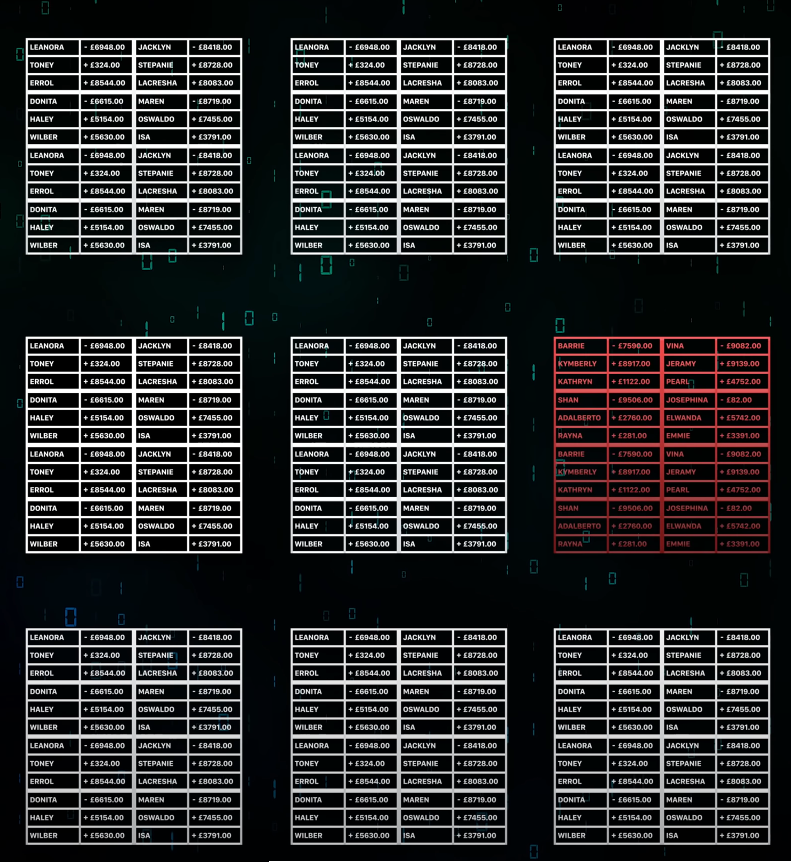
\includegraphics[scale=0.4]{slike/slika1.png}
\end{center}
\caption{Predstavljanje provere čvorova kada postoji kopija koja se ne poklapa}
\label{fig:proverakopija}
\end{figure}


Zbog toga su sve informacije u \emph{blockchain}-u ireverzibilne. U slučaju kriptovaluta, te informacije su liste transakcija, ali \emph{blockchain} može čuvati i druge vrste podataka, kao što su ugovori, lične karte ili inventar proizvoda kompanije.

Zbog decentralizovane prirode \emph{blockchain}-a, sve transakcije se mogu videti u okviru svoje kopije ili korišćenjem \emph{blockchain} pretraživača koji omogućavaju praćenje transakcija uživo. Svaki čvor ima svoju kopiju lanca koja se ažurira dodavanjem novih blokova. Ovo omogućava praćenje korišćenja kriptovalute. Ima slučajeva gde su razmene bile hakovane. Haker jeste ostao anoniman, ali je moguće pratiti korišćenje ukradene kriptovalute. Naravno, informacije u \emph{blockchain}-u su enkriptovane i samo vlasnik zapisnika može da dekriptuje podatke. Tako se održava anonimnost i transparentnost \cite{blockchain}.


\subsection{Sigurnost}
\label{subsec:sigurnost}
\emph{Blockchain} održava decentralizovanu sigurnost i poverenje na više načina. Za početak, blokovi se čuvaju linearno i hronološki, odnosno dodaju se na kraj lanca. To otežava vraćanje kroz lanac jer bi se promenile informacije u bloku, osim ako većina mreže to ne odobri. Svaki blok sadrži svoj heš, kao i heš bloka pre njega, slika \ref{fig:blockchain}. Heš se pravi od podataka u okviru bloka, pa ako dođe do promene neke informacije, promeniće se i heš.

\begin{figure}[h!]
\begin{center}
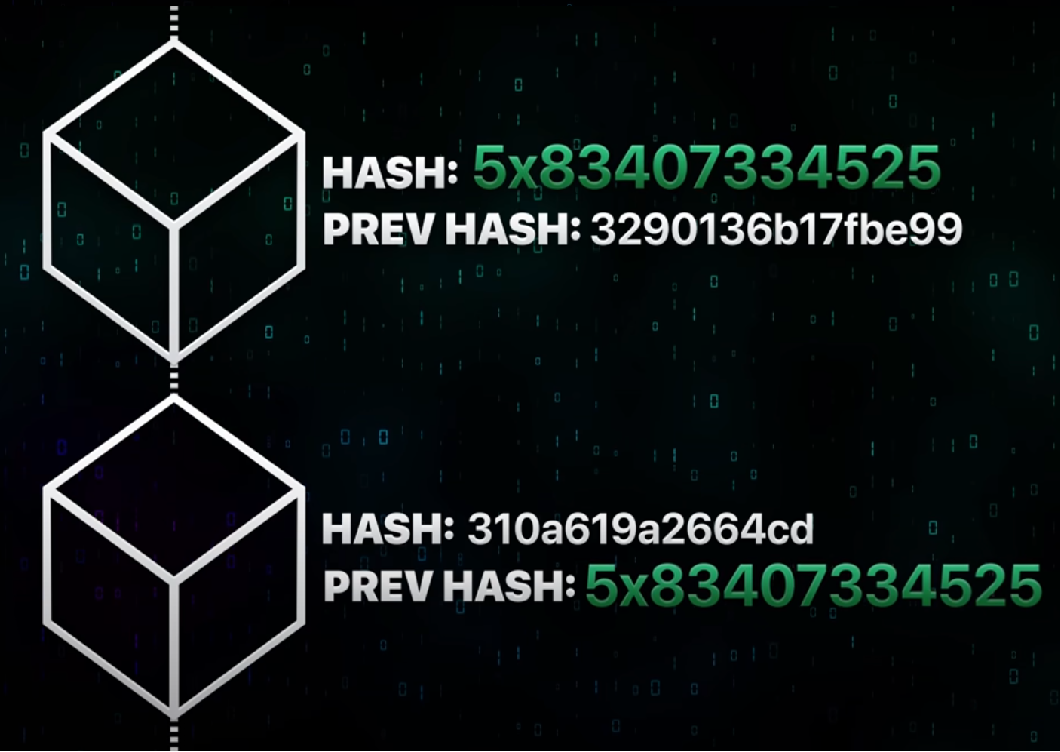
\includegraphics[scale=0.25]{slike/slika2.png}
\end{center}
\caption{\emph{Blockchain}}
\label{fig:blockchain}
\end{figure}


Ako haker, koji takođe ima čvor u mreži \emph{blockchain}-a, želi da promeni podatke i ukrade kriptovalutu od drugih, nije dovoljno da promeni samo svoju kopiju. Poređenjem sa ostalim kopijama će se primetiti odstupanje i ta kopija će se smatratiti nelegitimnom. Za uspešno hakovanje, potrebno je promeniti više od 50\% kopija. Takav napad bi zahtevao puno novca i sredstava jer bi morali promeniti svaki blok u lancu koji zbog promene imaju i promenjen heš \cite{blockchain}.


\subsection{\emph{Blockchain} kao tehnologija}
\label{subsec:tehnologija}
\emph{Stuart Haber} i \emph{W. Scott Stornetta} su istraživači koji su 1991. izmislili koncept \emph{blockchain}-a. Hteli su da implementiraju sistem u kome nije moguće menjati vremena dokumenata. Prošle su skoro dve decenije dok \emph{blockchain} nije dobio svoju upotrebu u stvarnom svetu sa pokretanjem \emph{Bitcoin}-a 2009. Ključnu stvar koju treba razumeti je da se  \emph{blockchain} u kriptovalutama koristi samo kao transparentni zapisnik plaćanja, ali u teoriji  se može koristiti za ireverzibilno zapisivanje bilo kog broja informacija. Te informacije mogu biti transakcije, glasovi za vreme izbora, inventari proizvoda, lične karte i mnogi drugi podaci.

Trenutno postoji mnogo projekata koji pokušavaju da implementiraju  \emph{blockchain} sisteme kako bi pomogli društvu. Jedan primer je sigurno glasanje na demokratskim izborima. Karakteristika nepromenljivosti podataka znatno otežava pokušaje lažnog glasanja. Sistem bi funkcionisao tako što bi svaki građanin dobio token. Kandidati bi imali svoje adrese novčanika i glasači bi slali svoje tokene na adresu kandidata za kojeg žele da glasaju. Karakteristike transparentnosti bi eliminisale potrebu za brojanjem glasova i mogućnosti praćenja tokena bi sprečile manipulisanje glasovima \cite{blockchain}.


\section{Tehnike verifikacije}
\label{sec:verifikacija}
Navedeno je da između čvorova mreže  \emph{blockchain}-a postoje provere koje verifikuju podatke, ali nismo ulazili u detalje. Te provere se odnose na jednu od dve tehnike validacije,  \emph{proof of wook} ili \emph{proof of stake}, koje se primenjuju nad transakcijama za sprečavanje prevara \cite{kriptovalute2}.

\subsection{\emph{Proof of wook}}
\label{subsec:work}
\emph{Proof of wook} je tehnika verifikacije gde algoritam generiše problem kog računari pokušavaju što pre da reše.
\emph{Miner} je naziv koji je pripisan svakom računaru koji učestvuje u rešavanju matematičkog problema koji pomaže pri verifikaciji grupe transakcija, koje predstavaljaju blok, i dodaje ih u  \emph{blockchain}. Prvi računar koji to uspešno uradi biva nagrađen malom količinom odgovarajuće kriptovalute.
Računari koji učestvuju u rešavanju problema rade u ponoj snazi dug vremenski period, što kod skupih računara generiše veliku potrošnju struje. To znači da  \emph{miner}-i jedva zarade nešto za validaciju transakcija kada uzmemo u obzir potrošnju i cenu samog računara \cite{kriptovalute2}.

\subsection{\emph{Proof of stake}}
\label{subsec:stake}
Neke kriptovalute koriste \emph{proof of stake} kao tehinku validacije da bi smanjili potrošnju energije potrebnu za proveru transakcija. Ovom tehnikom, broj transakcija koje korisnik može da odobri zavisi od količine kriptovalute koju je spreman da uloži, ili na neko vreme zaključa u komunalni sef, da bi imao šansu da učestvuje u procesu validacije.
Svako ko uloži kriptovalutu ima šansu da bude izabran za validaciju transakcije, ali šansa da neko bude izabran sa povećava sa većim ulogom.
Zato što \emph{proof of stake} ne zahteva intenzivna izračunavanja koja zahtevaju veliku količinu energije, znatno je efikasnije od \emph{proof of wook} i omogućava brza izvršavanja verifikacija ili potvrda transakcija.
Kao primer, vreme potrebno za transakciju kod \emph{Bitcoin}-a je u proseku najmanje 10 minuta, dok u poređenju \emph{Solana}, kripto platforma bazirana na \emph{proof of stake} tehnici, izvršava u proseku 3000 transakcija po sekundi.
Takođe, \emph{Ethereum}, \emph{Bitcoin}-ov najveći konkurent, u potpunosti prelazi na \emph{proof of stake} sistem \cite{kriptovalute2}.

Obe tehnike validacije se zasnivaju na mehanizmima konsenzusa. To znači da iako obe tehnike koriste pojedince za validaciju transakcije, one moraju biti proverene i odobrene od strane većine vlasnika kopija glavne knjige.\cite{kriptovalute2}


\section{Različite kriptovalute}
\label{sec:različitekriptovalute}

\subsection{\emph{Bitcoin}}
\label{subsec:bitcoin}
\emph{Bitcoin} je prva i ubedljivo najpopularnija kriptovaluta. Osnovan je 2009. od strane čoveka ili grupe pod pseudonimom \emph{Satoshi Nakamoto}. Dizajniran je da bude nezavisan od državne uprave ili centralne banke. Zavisi od  \emph{blockchain} sistema i kao tehniku verifikacije koristi \emph{proof of wook}. Popularnost \emph{Bitcoin}-a je tolika da je ogromno korišćenje energije, koje održavanje sistema zahteva, dovela u pitanje brigu o zagađenju životne sredine \cite{različitekriptovalute}.

\begin{figure}[h!]
\begin{center}
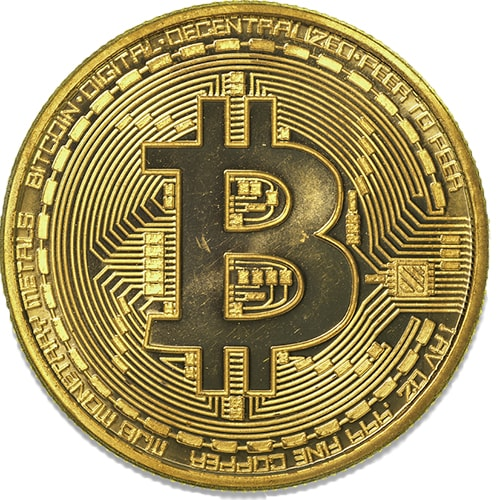
\includegraphics[scale=0.3]{slike/slika3.jpg}
\end{center}
\caption{\emph{Bitcoin} logo}
\label{fig:bitcoin}
\end{figure}


\subsection{\emph{Ethereum}}
\label{subsec:ethereum}
Kao \emph{Bitcoin}, \emph{Ethereum} je baziran na  \emph{blockchain} tehnologiji. Za razliku od \emph{Bitcoin}-a, dizajniran je kao programabilni  \emph{blockchain} odnosno nije napravljen da podrži samo valutu, nego najpre da omogući korisnicima mreže da prave, objavljuju i monetizuju decentralizovane aplikacije.  \emph{Ether}, izvorna valuta \emph{Ethereum}-a, napravljena je kao oblik plaćanja u okviru platforme. \emph{Ether} možemo posmatrati kao gorivo koje pokreće \emph{Ethereum}  \emph{blockchain}. \emph{Ethereum} je  \emph{blockchain} na kom je došlo do ogromnog zainteresovanja za \emph{NFT} o čemu će biti više priče u sledećem poglavlju.

Kao dva najpopularnija predstavnika, mnogo ljudi direktno poredi \emph{Bitcoin} i \emph{Ethereum} iako su napravljeni u dve različite svrhe. \emph{Bitcoin} je mreža za digitalni novac koja olakšava transakcije bez potrebe za centralnim autoritetom, dok \emph{Ethereum}, često nazivan računar sveta, baziran na tehnologiji \emph{Bitcoin}-a dodaje još i pametne ugovore (eng. \emph{smart contracts}). Oni omogućavaju pravljenje decentralizovanih aplikacija koje obuhvataju širok spektar programa. \emph{Ethereum} takođe koristi \emph{proof of wook} kao sistem za validaciju, ali kao što je već navedeno, planiraju da pređu na \emph{proof of stake} sistem. Još jedna razlika je što je \emph{Bitcoin} ograničen na 21 milion jedinica \emph{Bitcoin} tokena, dok je \emph{Ether} neograničen \cite{različitekriptovalute}.


\begin{figure}[h!]
\begin{center}
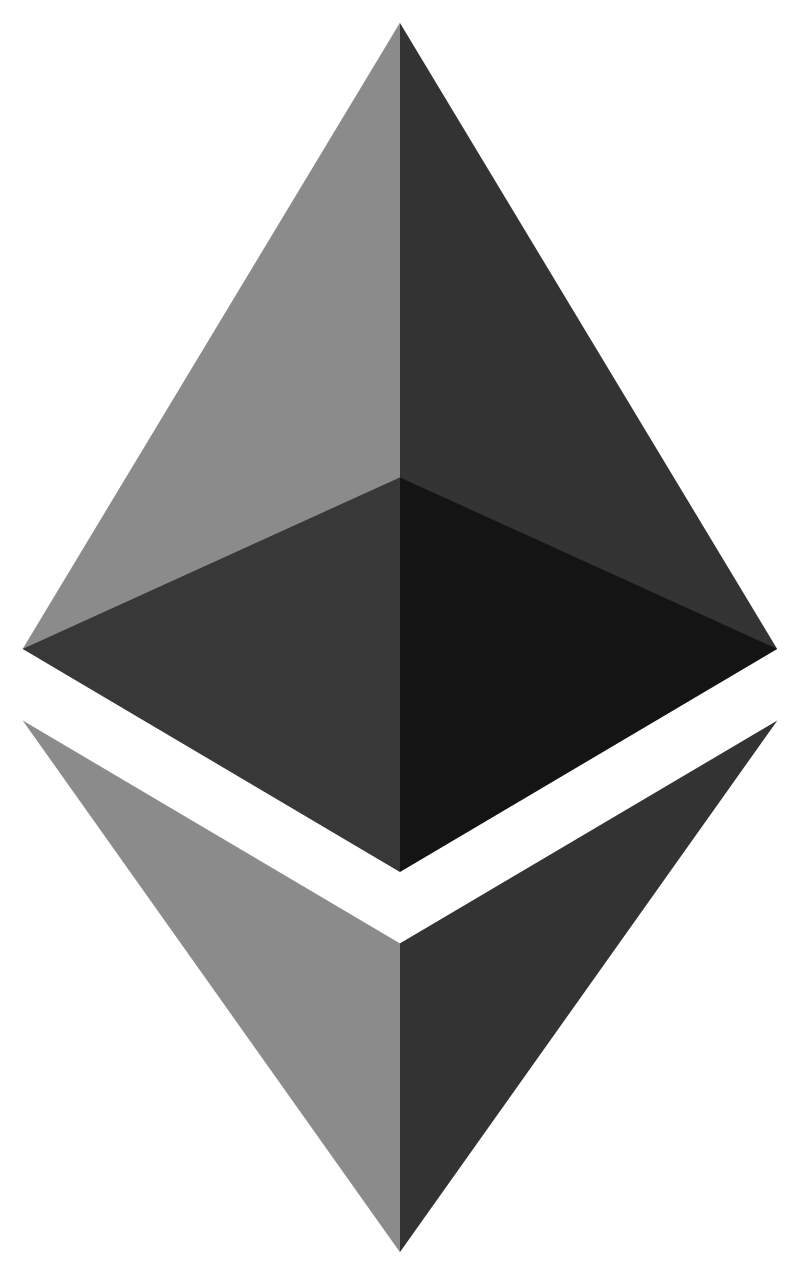
\includegraphics[scale=0.1]{slike/slika4.png}
\end{center}
\caption{\emph{Ethereum} logo}
\label{fig:ethereum}
\end{figure}


\subsection{\emph{Cardano}}
\label{subsec:cardano}
\emph{Cardano} je  \emph{blockchain} platforma sa \emph{proof of stake} sistemom verifikacije koja ima funkcionalnosti pametnih ugovora. \emph{Cardano} je poznat po svom fokusu na akademska istraživanja, velikoj propusnosti transakcija u sekundi i energetski efikasnom konsenzus mehanizmu \emph{Ouroboros}. \emph{Cardano} je izvorna valuta \emph{Cardano} mreže i služi da olakša transakcije i izvršavanje pametnih ugovora. \emph{Ada Lovelace}, matematičarka 19. veka, je inspiracija za naziv valute. \emph{Cardano} se razvija u pet faza ka postizanju cilja razvijanja mreže u platformu decentralizovanih aplikacija. Svaka faza u planu zasnovana je na istraživačkim okvirima i recenziranim uvidima koji su pomogli za uspostavljanje akademske reputacije.\cite{različitekriptovalute}

\begin{figure}[h!]
\begin{center}

\includegraphics[scale=0.4]{slike/slika5.png}
\end{center}
\caption{\emph{Cardano} logo}
\label{fig:cardano} 
\end{figure}


\newpage

\section{\emph{Non-fungible token (NFT)}}
\label{sec:nft}
\textbf{Zamenljivost (eng. \emph{Fungibility})} znači da je nešto moguće zameniti nečim indentičnim. Kada je nešto zamenljivo, tipično ih je mnogo istih. Zamenljiv token se može podeliti i zemeniti za neki drugi.

\textbf{Nezamenljivost (eng. \emph{Fungibility})} nudi jedinstvenost kao glavni atribut. Nezamenljiv token je jedinstven i ne može postojati još jedan isti. Kao primer, avionska karta je jedinstvena, odnosi se na određeno mesto, određeni let u određeno vreme.

Nezamenljiv token (eng. \emph{NFT}) je tip kriptografskog tokena koji predstavlja jedinstvenu stvar. Te stvari mogu biti digitalne ili fizičke. Nezamenljivi tokeni omogućavaju vlasnicima da dokažu vlasništvo i autentičnost neke stvari. Takođe olakšava proces kupovine preduzećima ili pojedincima jer mogu da veruju da će dobiti ono što su kupili zbog provere identifikatora nezamenljivog tokena te stvari \cite{nft}. Karakteristike nezamenljivih tokena:\\ 

\textbf{Nedeljivost:} Oni se ne mogu podeliti kada je u pitanju njihova funkcionalnost. Avionska karta se ne može iskoristiti nekim njenim delom već samo u celosti, jer se odnosi samo na jedno mesto koje samo jedna osoba može da iskoristi.\\ 

\textbf{Retkost:} Nedeljivi tokeni mogu biti retki i to je nešto što im daje vrednost. Iako je moguće generisati mnogo sredstava, tako je isto moguće limitirati broj tokena.\\

\textbf{Jedinstvenost:} Jedinstveni su jer ne postoje dva ista nezamenljiva tokena. Metapodaci nezamenljivih tokena su nepromenljivi zapisi koji im daju sertifikate autentičnosti.\\

\textbf{Vlasništvo:} Žive u \emph{blockchain}-u u okviru nečijeg računa. Kreatori nezamenljivog tokena kontrolišu privatni ključ računa u kom se nalazi i imaju slobodu da ga prebace na nečiji račun.\\

\textbf{Transparentnost:} Zbog karakteristika  \emph{blockchain}-a gde zapisi izdavanja, transfera i aktivnosti nekog tokena mogu biti javno verifikovani, kupci mogu da veruju i verifikuju autentičnost nekog željenog tokena.\\

\textbf{Kompatibilnost:} Nezameljivi tokeni se mogu zameniti, kupiti ili prodati preko različitih  \emph{blockchain} sistema, koristeći decentralizovani most ili centralizovane službe.


\newpage


\section{Zaključak}
\label{sec:zaključak}
Iako kriptovalute imaju mnogo prednosti, kao što su brza internacionalna plaćanja bez brige o kursevima valute i bez ograničenja, nisu ni one savršene. Ako bi se u potpunosti prešlo na sistem kriptovaluta, najveći izazov predstavlja određivanje poreza koji je bitan za razne aspekte funkcionisanja države. Problem je još što iako je  \emph{blockchain} siguran sistem, moguće je izvršiti hakerske napade na digitalne novčanike koji nisu deo sistema. Ali najveći problem predstavlja određivanje vrednosti.

Ne postoji ništa na osnovu čega bi se odredila tačna vrednost kriptovalute, sve su samo spekulacije. Vrednost se trenutno određuje time koliki je nivo zainteresovanosti ljudi i koliko su spremni da ulože. Za uspešno ulaganje je potrebno veliko razumevanje samog sistema i ekonomije, što prosečan stanovnik nema, a zbog velike popularnosti može da se uključi u celu priču i potencijalno sebi napravi štetu. Zbog trenutne krize i situacije u svetu, vrednost kriptovaluta je opala na najniži nivo posle dugog perioda uzastopnog rasta.

Ono što jeste bitno je tehnologija na kojoj je sve bazirano. Internet je primer tehnologije koji se drastično promenila u poređenju na prve oblike i koji nastavlja da se razvija.  \emph{Blockchain} ima dobre karakteristike koje su privukle veliku pažnju. Tako da, iako sada nisu prisutni svuda, mogu postati deo svakodnenog života i to u nekom potupno drugom obliku.

\addcontentsline{toc}{section}{Literatura}
\appendix

\iffalse
\bibliography{literatura} 
\bibliographystyle{plain}
\fi

\begin{thebibliography}{9}

\bibitem{kriptovalute1}
\href{https://www.kaspersky.com/resource-center/definitions/what-is-cryptocurrency}{\emph{What is cryptocurrency and how does it work? Kaspersky.}}

\bibitem{istorijabitcoina}
\href{https://money.usnews.com/investing/articles/the-history-of-bitcoin}{\emph{Wayne Duggan. The History of Bitcoin, the First Cryptocurrency, 2022.}}

\bibitem{istorijanovca}
\href{https://www.investopedia.com/articles/07/roots_of_money.asp}{\emph{Andrew Beattie,  Caitlin Clarke. The History of Money, 2022}}

\bibitem{kriptovalute2}
\href{https://www.forbes.com/advisor/investing/cryptocurrency/what-is-cryptocurrency/}{\emph{Kate Ashford, 
Farran Powell. What Is Cryptocurrency? 2022.}}

\bibitem{blockchain}
\href{https://www.investopedia.com/terms/b/blockchain.asp}{\emph{Adam Hayes,  Jefreda R. Brown, Suzanne Kvilhaug. Blockchain Facts: What Is It, How It Works, and How It Can Be Used, 2022.}}

\bibitem{različitekriptovalute}
\href{https://www.sofi.com/learn/content/understanding-the-different-types-of-cryptocurrency/}{\emph{Carla Tardi. Understanding the Different Types of Cryptocurrency, 2022}}

\bibitem{nft}
\href{https://hedera.com/learning/tokens/what-is-a-non-fungible-token-nft?adgroupid=139332525739&utm_term=&utm_campaign=hh19c1&utm_source=sem&utm_medium=ppc&utm_content=611328684444&hsa_acc=1782665900&hsa_cam=1717906681&hsa_grp=139332525739&hsa_ad=611328684444&hsa_src=g&hsa_tgt=dsa-1692334474972&hsa_kw=&hsa_mt=&hsa_net=adwords&hsa_ver=3&gclid=EAIaIQobChMIkarYjMSS-gIVkAwGAB2K9gOcEAAYAyAAEgJqcPD_BwE}{\emph{What is a non-fungible token (NFT)? Hedera.}}





\end{thebibliography}


















\end{document}